\documentclass{article}
\usepackage{listings}
\usepackage{mathrsfs}
\usepackage[utf8]{inputenc}
\usepackage{amssymb}
\usepackage{lipsum}
\usepackage{amsmath}
\usepackage{fancyhdr}
\usepackage{geometry}
\usepackage{scrextend}
\usepackage[english,german]{babel}
\usepackage{titling}
\setlength{\droptitle}{-3cm}
\usepackage{tikz}
\usepackage{algorithm,algpseudocode}
\usepackage[doublespacing]{setspace}
\usetikzlibrary{datavisualization}
\usetikzlibrary{datavisualization.formats.functions}
\usepackage{polynom}
\usepackage{amsmath}
\usepackage{gauss}
\usepackage{tkz-euclide}
\usepackage{minted}
\usepackage{mathrsfs}
\usetikzlibrary{datavisualization}
\usetikzlibrary{datavisualization.formats.functions}
\author{
Alexander Mattick Kennung: qi69dube\\
Kapitel 1
}
\usepackage{import}
\date{\today}
\geometry{a4paper, margin=2cm}
\usepackage{stackengine}
\parskip 1em
\newcommand\stackequal[2]{%
  \mathrel{\stackunder[2pt]{\stackon[4pt]{=}{$\scriptscriptstyle#1$}}{%
  $\scriptscriptstyle#2$}}
 }
\makeatletter
\renewcommand*\env@matrix[1][*\c@MaxMatrixCols c]{%
  \hskip -\arraycolsep
  \let\@ifnextchar\new@ifnextchar
  \array{#1}}
\makeatother
\lstset{
  language=haskell,
}
\lstnewenvironment{code}{\lstset{language=Haskell,basicstyle=\small}}{}
\usepackage{enumitem}
\setlist{nosep}
\usepackage{titlesec}
\usepackage{ stmaryrd }
\usepackage{verbatim}
\usepackage{tikz-qtree}
\usepackage{bussproofs}

\titlespacing*{\subsection}{0pt}{2pt}{3pt}
\titlespacing*{\section}{0pt}{0pt}{5pt}
\titlespacing*{\subsubsection}{0pt}{1pt}{2pt}
\title{Übung 7}


\begin{document}
	\[P=\begin{bmatrix}2a&0&2b&0\\0&2/5&0&3/5\\3a&0&1/6&b\\0&3/5&0&2/5 \end{bmatrix}\]
	bestimme a,b)\\
	Zeilensumme muss eins sein und alle Einträge positiv.\\
	\[\begin{bmatrix}2&2\\3&1\end{bmatrix}(a,b)^T = \begin{bmatrix}1\\5/6\end{bmatrix}\]
	$b=1/3, a=1/6$
	\[P=\begin{bmatrix}1/3&0&2/3&0\\0&2/5&0&3/5\\1/2&0&1/6&1/3\\0&3/5&0&2/5 \end{bmatrix}\]
	(self-loops sin wichtig in NNs: sie erlauben den Neuronen sich an dinge zu erinnern, also RNN/GRU/LSTM dort aber mit einem delay. Okay Yamakou redet stattdessen über Graph NN's, Deep ODNs etc, JETZT nimmt er das triviale reinforcement learning beispiel)\\
	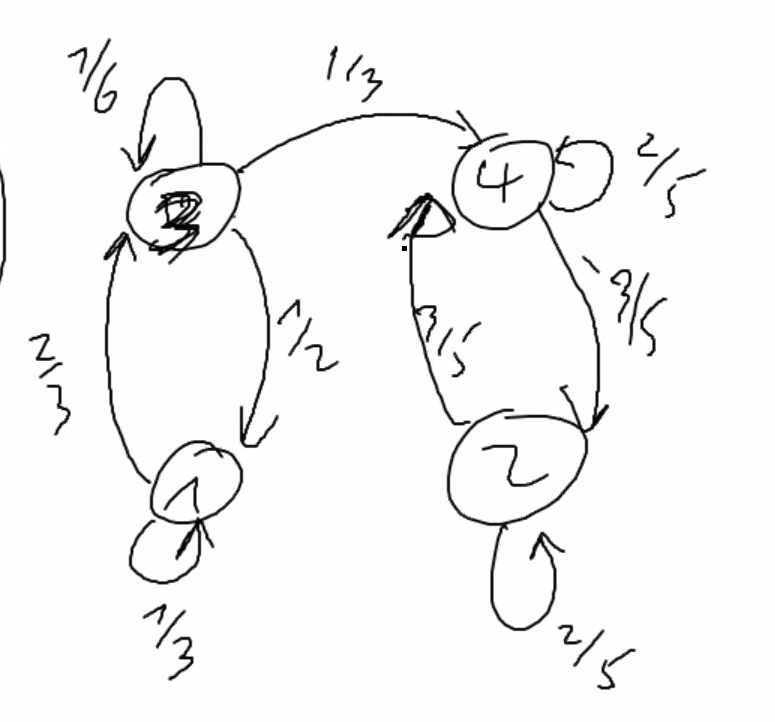
\includegraphics{graph.png}\\
	gleichgewicht:\\
	$\pi P = \pi$ somit ist $\pi$ ein linkseigenvektor von P.\\
	$\pi P-\pi = 0\iff \pi(P-I)=0 \iff \pi(P-I)^T =0\iff (P^T-I)\pi^T =0$ also Reduktion auf rechtseigenvektor.\\
	\[det(\begin{bmatrix}1/3&0&2/3&0\\0&2/5&0&3/5\\1/2&0&1/6&1/3\\0&3/5&0&2/5 \end{bmatrix}^T -\lambda I)v=0\]
	\[P^T = \begin{bmatrix}1/3&0&1/2&0\\0&2/5&0&3/5\\2/3&0&1/6&0\\0&3/5&1/3&2/5 \end{bmatrix}\]
	für uns ist nur der EW von $\lambda = 1$ relevant, somit
	\[\begin{bmatrix}1/3-1&0&1/2&0\\0&2/5-1&0&3/5\\2/3&0&1/6-1&0\\0&3/5&1/3&2/5-1 \end{bmatrix}\]
	jetzt lösen
	\[\begin{bmatrix}
	-2/3&0&1/2&0\\
	0&-3/5&0&3/5\\
	0&0&-1/3&0\\
	0&0&1/3&0 \end{bmatrix}\]
	\[\begin{bmatrix}
	-2/3&0&1/2&0\\
	0&-3/5&0&3/5\\
	0&0&-1/3&0\\
	0&0&0&0 \end{bmatrix}\]
	davon der Kern ist der EV, man muss diesen nun normiert aufschreiben $(0,\frac{1}{\sqrt{2}},0,\frac{1}{\sqrt{2}})$\\



\end{document}
